\documentclass[11pt]{article}
\renewcommand{\baselinestretch}{1.8}
\usepackage{textcomp}
\usepackage{fontenc}
\usepackage{graphicx}
\usepackage{caption} % for Fig. captions
\usepackage{gensymb} % for \degree
\usepackage{placeins} % for \images
\usepackage[margin=1in]{geometry} % to set margins
\usepackage{setspace}
\usepackage{lineno}
%\usepackage{cite}
\usepackage{amssymb} % for math symbols
\usepackage{amsmath} % for aligning equations
\usepackage[sort&amp;compress]{natbib}
\usepackage{xr-hyper}


\linenumbers



\date{}
\author{D.M. Buonaiuto $^{1,2,a}$, E.M. Wolkovich$^{3}$}

\begin{document}
\maketitle
\section*{Introduction}

\begin{enumerate}
\item Competition among plants in determined by a combination of intrinsic (growth rate, rooting depth, nutrient uses) and extrinsic (micro habitat, density dependence, founder effects) properties. 
\item In temporally variable environments, climate variability mediates all these processes which allows for coexistance.
\item Climate change will effect these dynamics, and a major effort of community ecology in an era of global change is to anticipate howa changing environment will effect these species interactions.
\item There is evidence that competition in the early stages of plant ontogeny (``regeneration niche" might be particularly effected).
\item Observation in dry grasslands tell us that ``storage effect dynamics" and ``seasonal priority effects" are importan \citep{Rudolf:2019a}.
\item We also see that climate change might amplify the impotance of these processes. 

\item However, we don't know how important these temporal dynamics are in temperate forest species. 
\item Several barriers:
\begin{enumerate}
\item Unlike dryland where water avialability is the primary determinant of germination, in temperate forest there are 2 (stratification x incubation)
\item Not alot of annuals. Which means:a) hard to measure fitness. b) hard to study seed emergence (is it a seed or a ramet?) c) competition between ramets may be historically more important but seeds matter for colonizing new areas and shifting do to climate change,
\end{enumerate}
\item However we can understand the role of these dynamics by characterizing regernation niches of species in contolled environemnts and applying them in current and future climate scenarios.
\item We do this.
\end{enumerate}

\section*{Here's the points of the paper}
\begin{enumerate}
\item We observed the response to a lot of different strafication regimes and 2 incubation temperatures for 3 temperate herbs as a case study and then modeled things in a bunch of different ways. We compare a day of change in stratification to a degree of change in warming and find that a the effect of one degree of warming is about 5x of 1 day of change (make plot or table of model results)....but....
\item  Re-analyzing soil warming experiments we calculate how much stratification is supposed to change. Answer from Harvard Forest means 79.2 to 47.3 but sd's around 26. That's with just 2.5 degrees warming How does this impact species.?

\item Then we projected germination percentages under current and future climate scenarios based on the above measurements from Harvard Forest (Fig. \ref{fig:germpercs}). We see that the 5 degree incubation differences dont matter nearly as mich as the loss of stratification.

\item Because its not only aboslute germination \% that affects competions but also timoing of germination Also we used a survivial model to figure out when each species reach (Fig. \ref{fig:germtime}). Here too, we see that stratification is the driver.

\item But Dan, these projections are just based on means. There is a ton of interannual variation in both scenarios. What about the storage effect? Couldn't that stabalize or equlize dynamics? If you simulate 100 years of variaiton under both scenarios, your figure from plot 1 looks quite different (Fig. \ref{fig:germpercswvar}).
    
    \item Granted but lets think if it a differnt way. How often is germination incomplete in each scenario? Very different pictures (Fig. \ref{fig:germfreq}). This might make the storage effect way more important.
    \end{enumerate}
    
\section{A TON of caveats}
\begin{itemize}
\item we didn't actually measure competion just relying on the literature to say that propgule pressue and priority effects matter.
\item Interannual variation might change with climate change too
\item We aren't trying to say much about these specific species (we don't know about their seed banks, or competitive interactions, or the fact they compete with hungred of others in the wild, or their seeds are often competing with vegetative propegations) but are using them to illustrate temporal dynamcis could become more important with climate change as it highlights differences in the response of species to change environments.
\item this is especially prevelant in chilling. We assume chilling was usually met in the past for all species and will be met less often in the future. 
\item Overall, our study just show we need to thing about these dynamics in temperate forests. Do we really buy that?
\end{itemize}

\section{Figures}

\begin{figure}[h!]
        \centering
        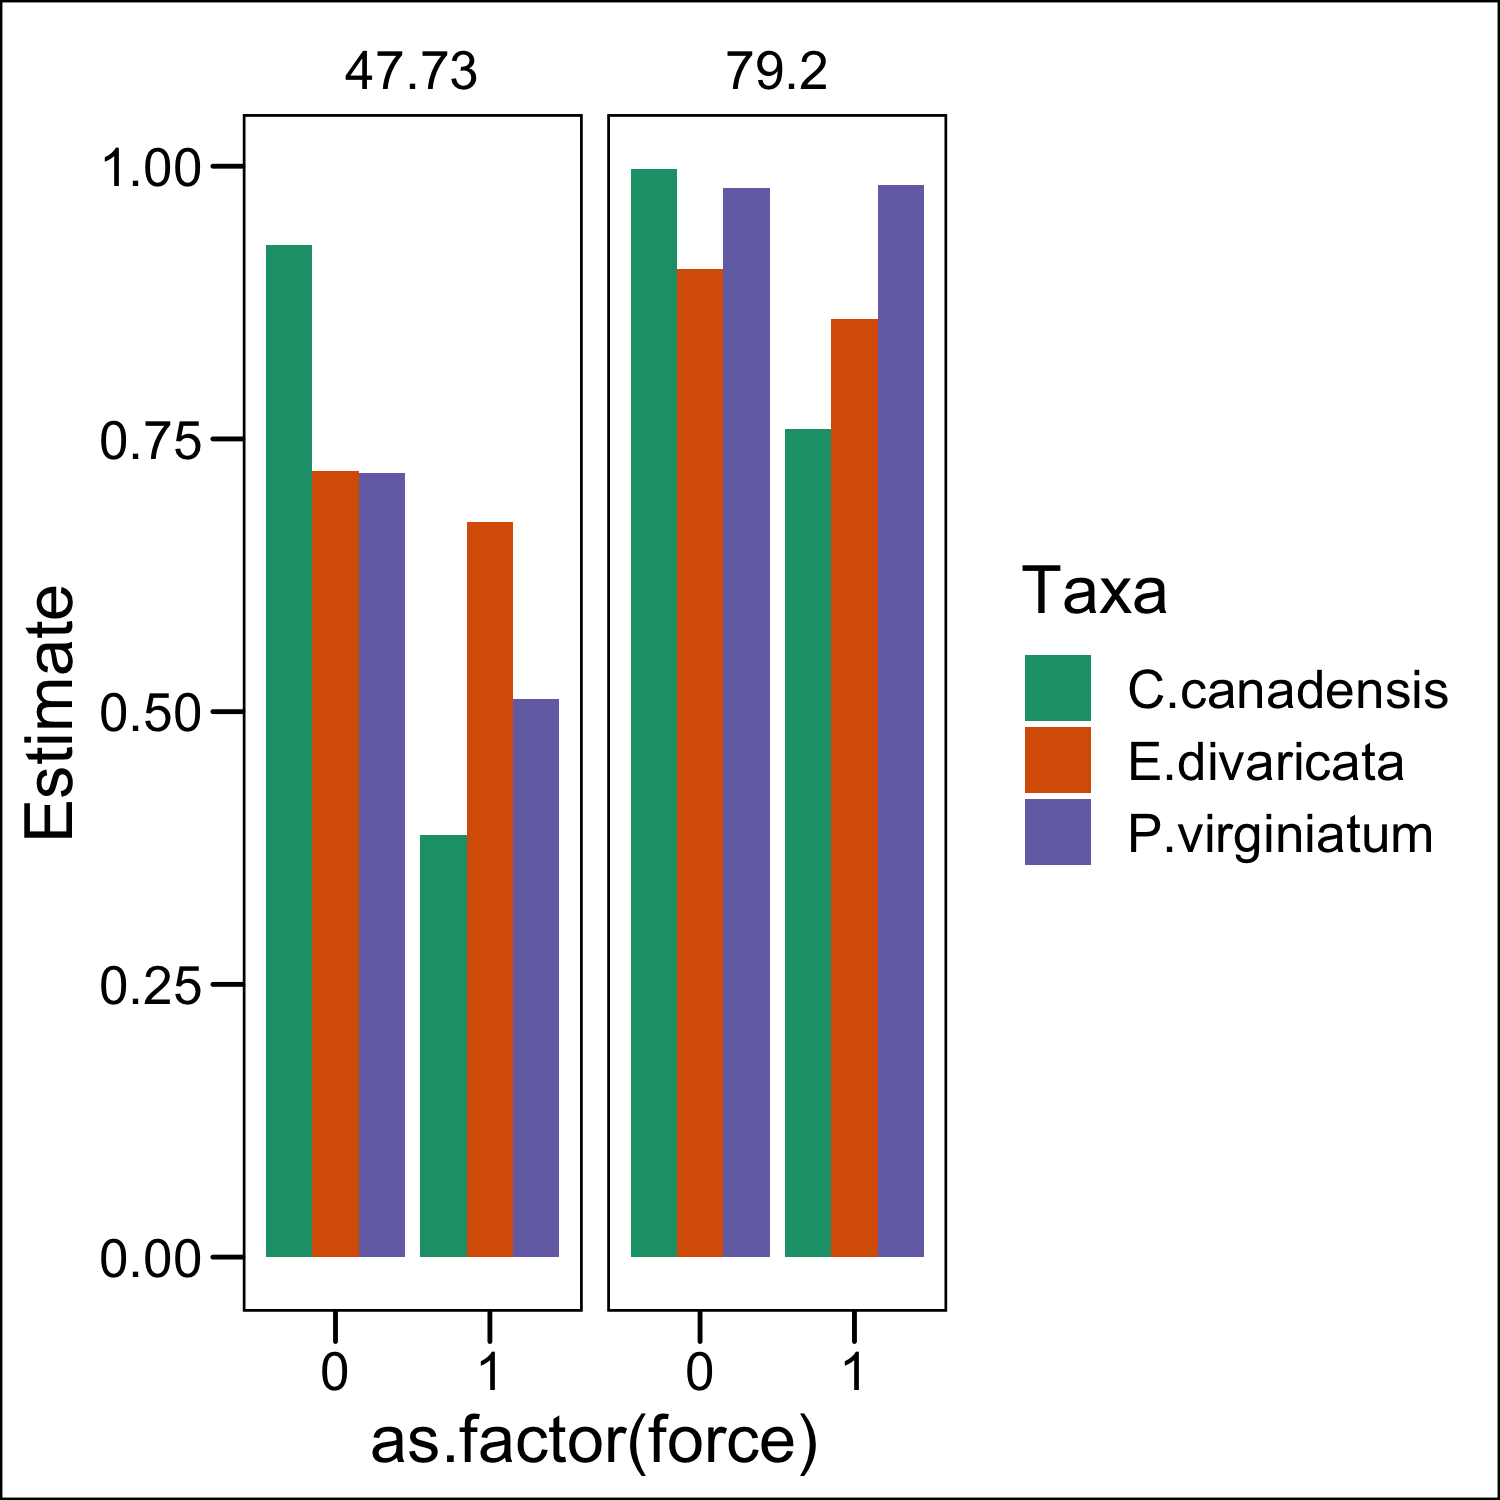
\includegraphics[width=0.8\textwidth]{..//figures/germpercs.png}
          \caption{Under ambient conditions (79.2/0, all species germinat above 80\%. This gets worse with warming, and way worse when chilling goes down and warming.}
        \label{fig:germpercs}
    \end{figure}

\begin{figure}[h!]
        \centering
        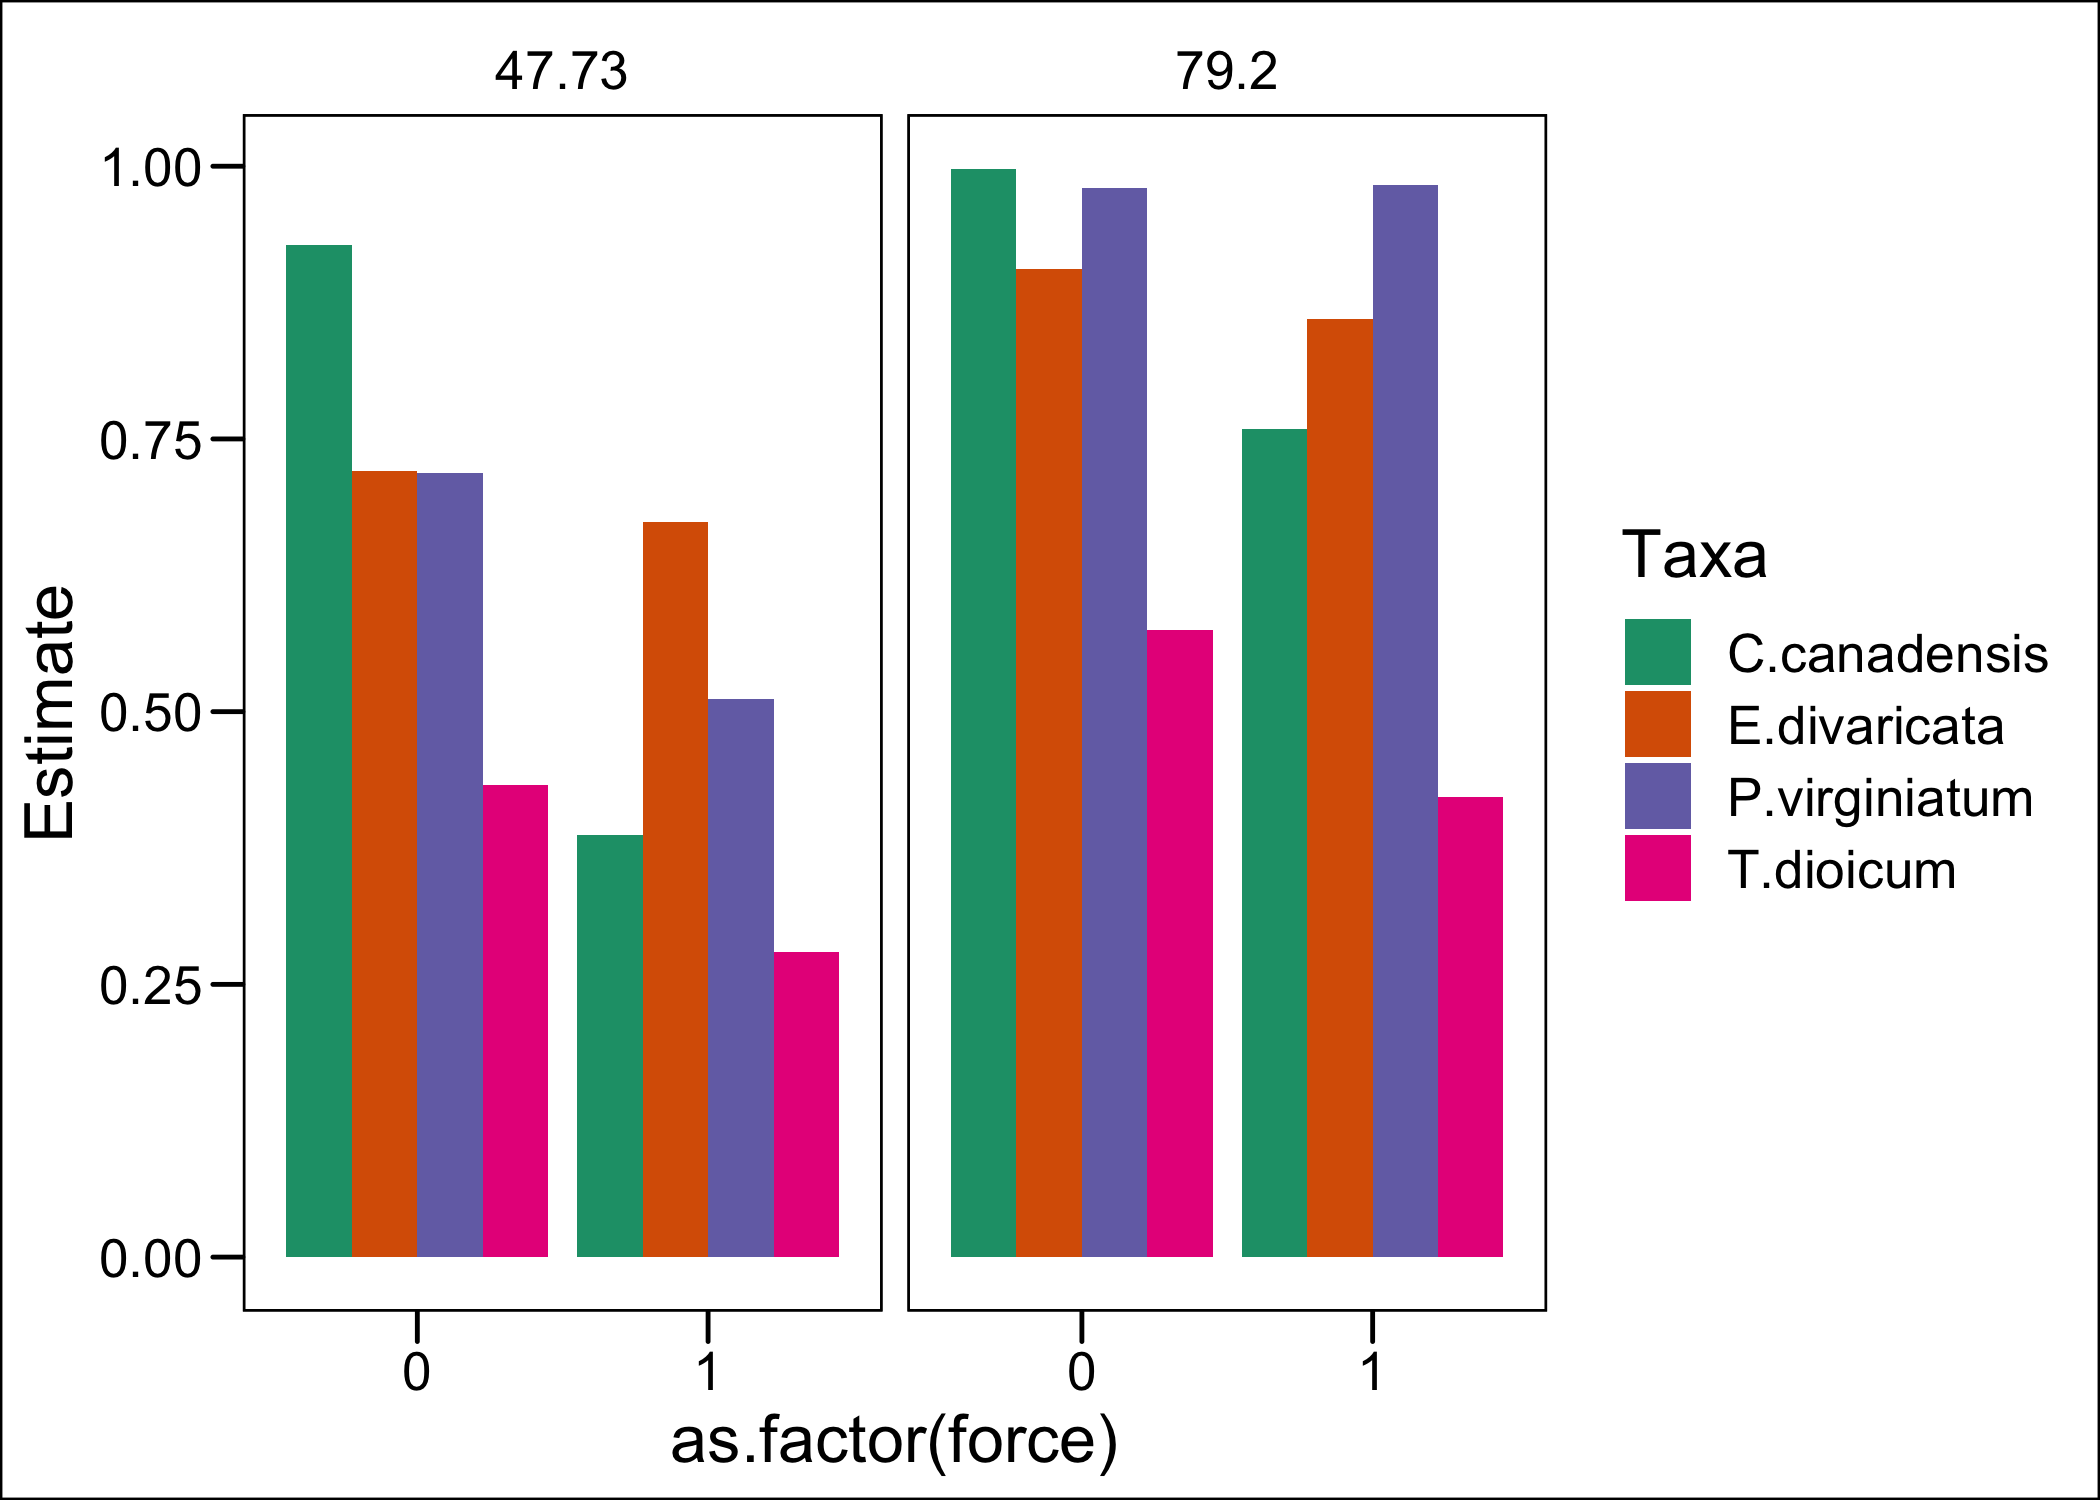
\includegraphics[width=0.8\textwidth]{..//figures/germtime.png}
          \caption{Look the timing of germination also gets spread amoung species with climate change, which likely will amplify priority effects}
        \label{fig:germtime}
      
  \end{figure} 
  
  \begin{figure}[h!]
        \centering
        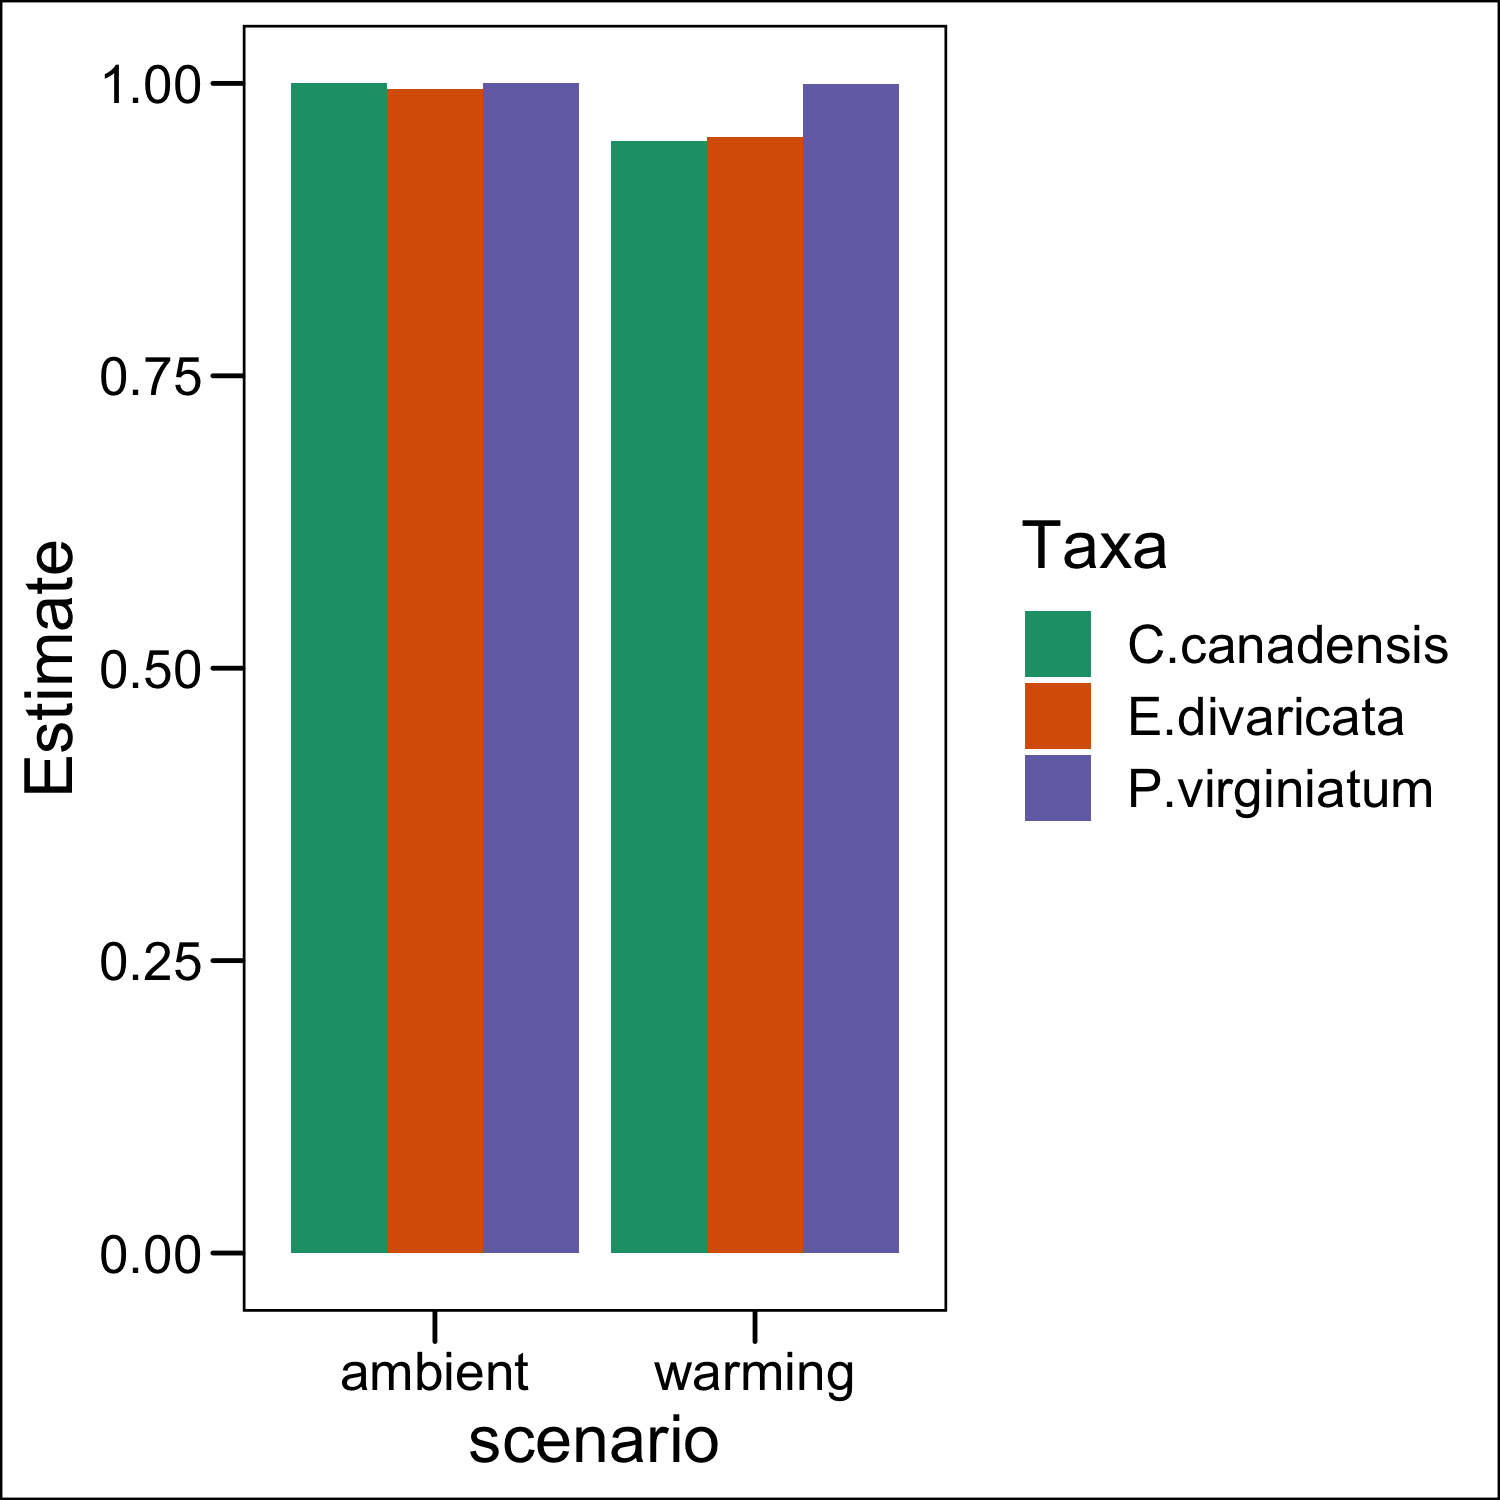
\includegraphics[width=0.8\textwidth]{..//figures/germpercs_wvar.png}
          \caption{Over 100 year the mean germination percentages aren't that different if the variation stays similar}
        \label{fig:germpercswvar}
    \end{figure}
    
        \begin{figure}[h!]
        \centering
        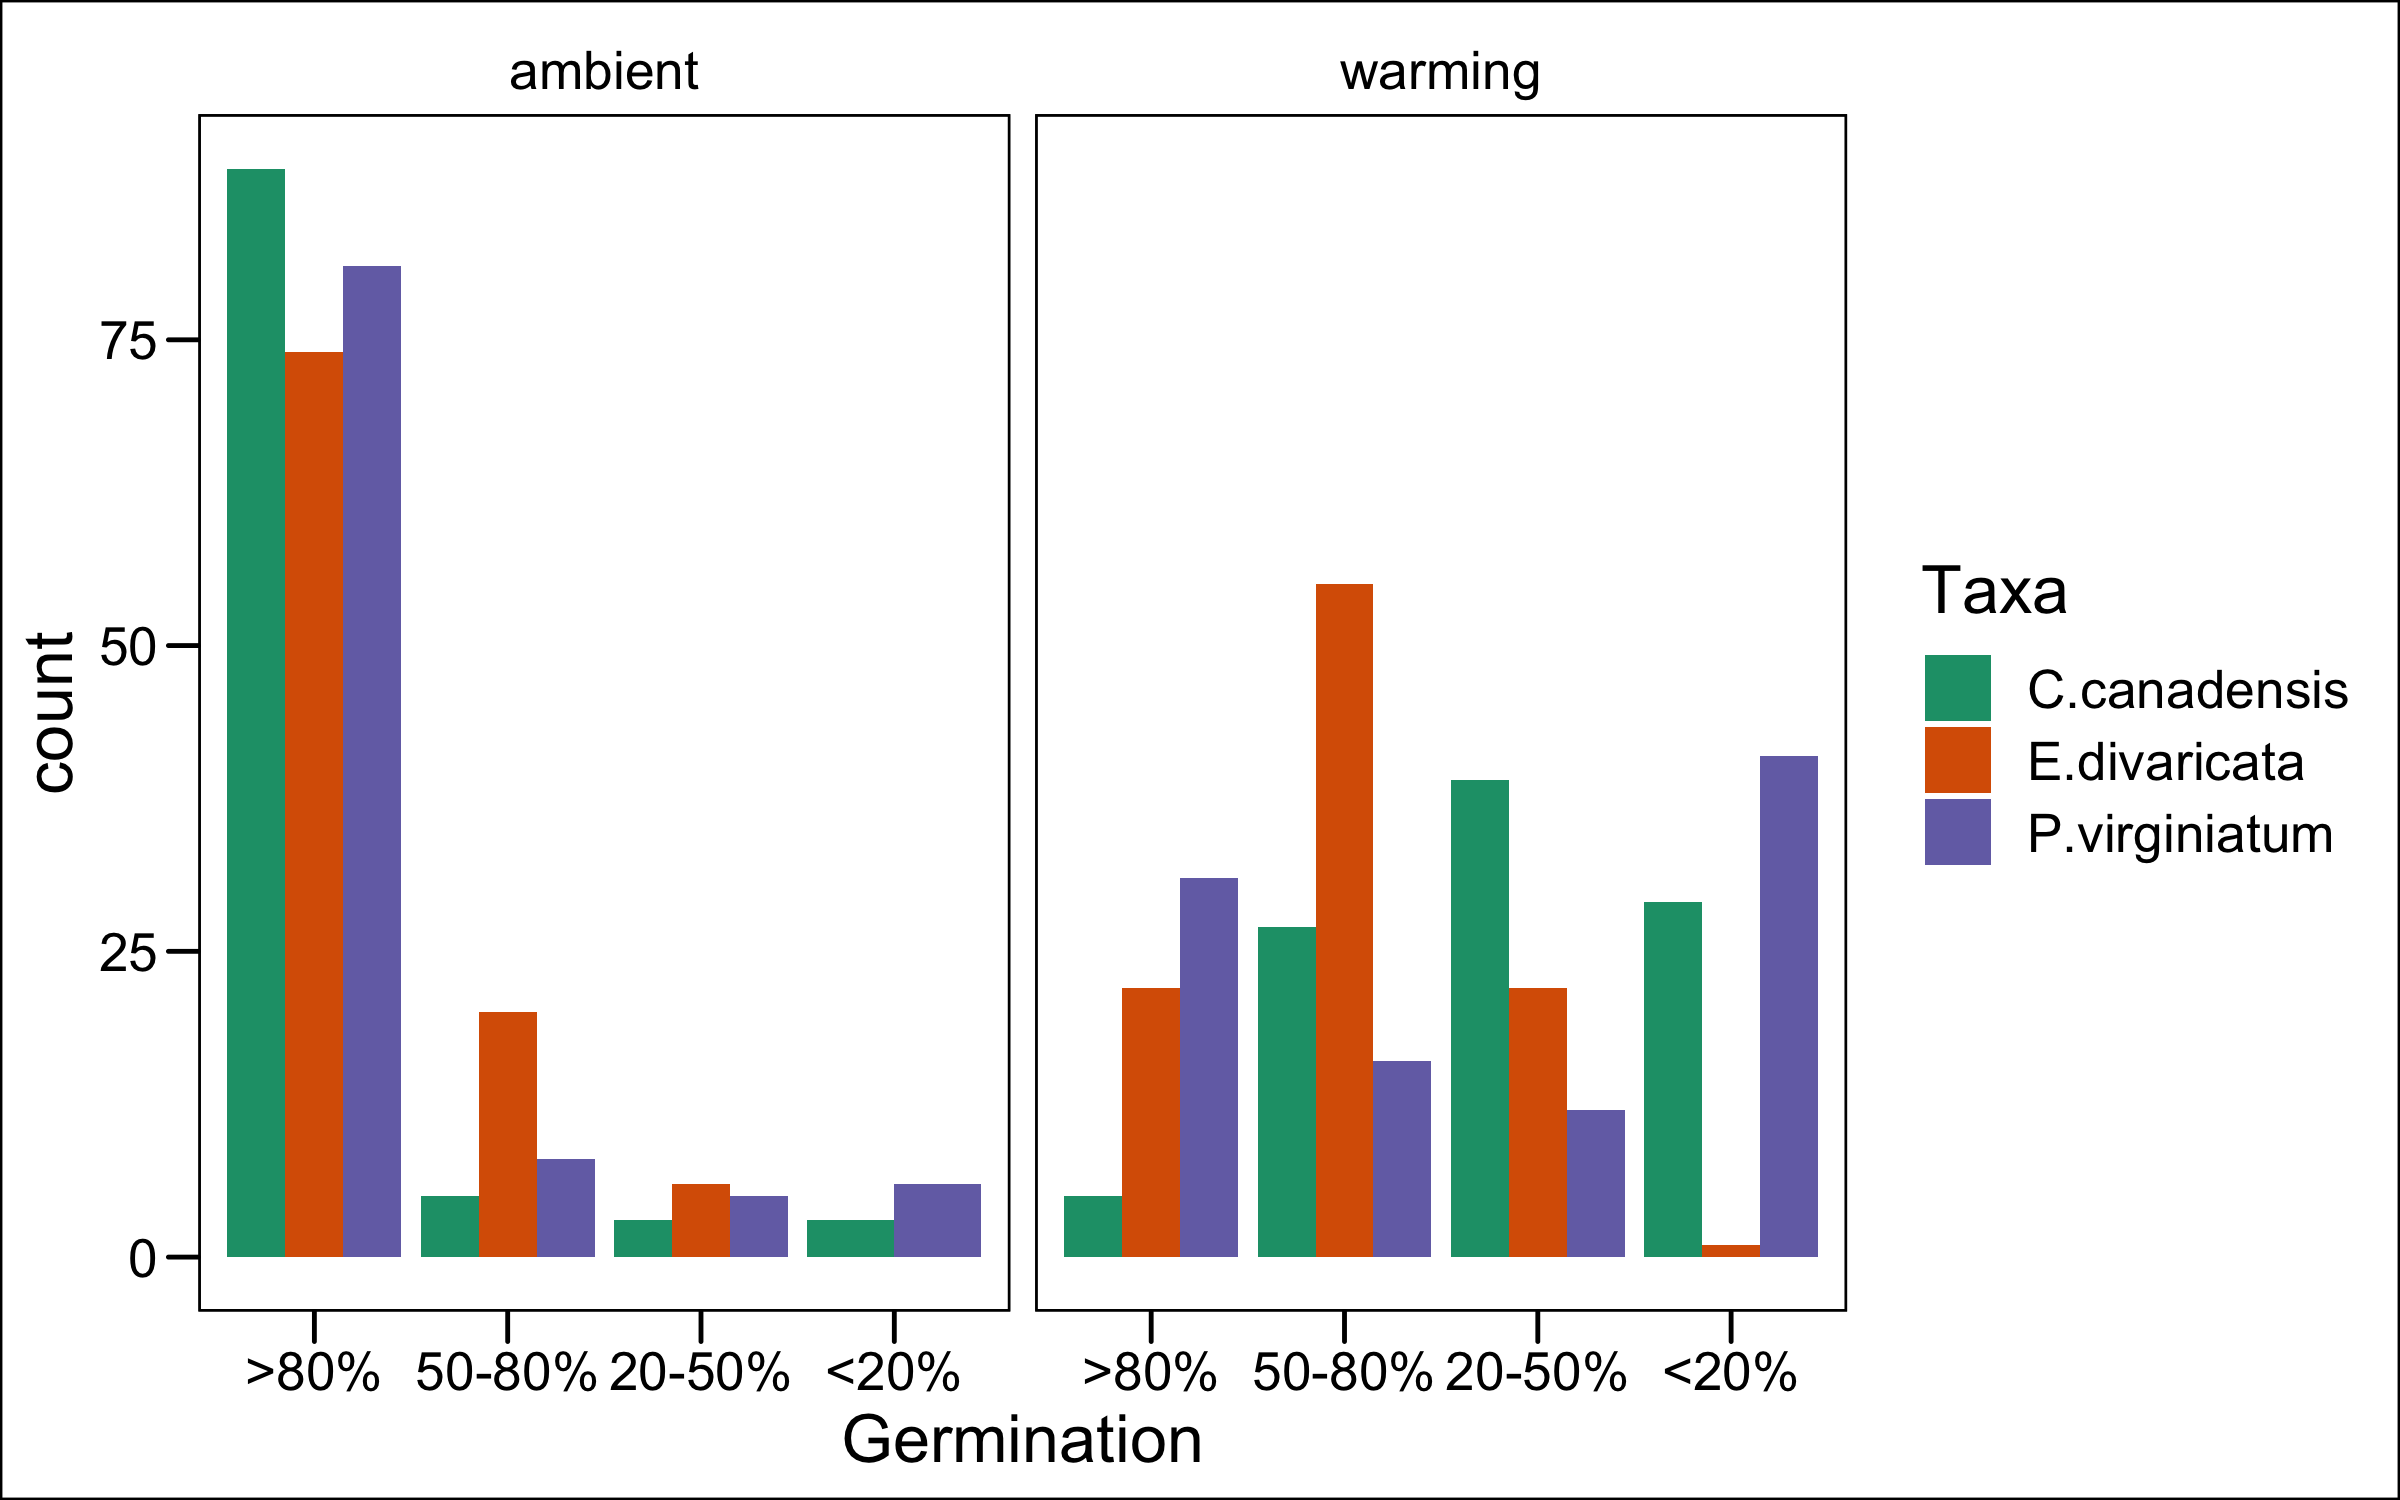
\includegraphics[width=0.8\textwidth]{..//figures/germfreq.png}
          \caption{The years in which there is good germination go way down for all species, but different. If they seedbank this could make for some intense storage effect dynamics}
        \label{fig:germfreq}
    \end{figure}

  \end{document}  

